\chapter{Problem Formulation}
\label{sec:chapter3}
\thispagestyle{empty}

This chapter formulates the problem we investigate in this thesis, namely doors detection in autonomous mobile robots. We start by discussing the usefulness of door detection for robotics applications, reporting some challenging tasks for autonomous agents, and how they can benefit from door detection. Next, we formally define the goal addressed by this thesis. The first one is the creation of a doors detector for mobile robots using an end-to-end technique. The second is a technique to improve the detector's performance in a certain deployment scenario, by exploiting the structural features of indoor environments. This work also tries to overcome some limitations of Deep Learning applied to robotics, such as the lack of datasets and metrics suitable for robotics applications. We proceed defining the concept of doors and the ideal deployment scenario considered by our work. Finally, we report the solutions adopted by this thesis.

\section{The Utility of Doors Detection for Mobile Robots}

As mentioned in the previous chapter, doors are useful semantic features for an active agent. By collecting information about doors, a robot can improve significantly its knowledge about the environment in which it operates. Exploration and navigation, two of the main tasks performed by a mobile robot, can be strongly influenced by exploiting knowledge about doors, such as their location and status (e.g. closed or opened). 

Exploration is the task in which an autonomous agent incrementally discovers features of interest in an initially unknown environment. Typically, an autonomous agent builds a map of the environment to perform navigation.  Map acquisition enables autonomous agents to navigate inside a previously unknown environment. With this procedure, a robot builds a metric map of the indoor environment it is exploring. A metric map is represented by an occupancy grid: a two-dimensional matrix in which each cell represents a sub-portion of the environment and contains the probability that the portion is occupied by an obstacle or it is free. Occupancy grids were first proposed in \cite{cuupancygridfirst} and they have become widely used for mobile robot localization, exploration, and navigation \cite{gridmapnavigation, ariel, girdmapexploration}. A way to store and visualize occupancy grid maps is to encode them in an 8-bit gray-scale image, normalizing the probability values of the cells to the range between 0
and 255. A further simplification in the binary occupancy grids (Fig. \ref{fig:binary_grid_map}), where each cell has a boolean value representing the occupancy status. An occupied location is represented as \textit{True} (1) while free spaces are tagged with \textit{False} (0). Collecting data about doors can improve the mapping strategy followed by mobile robots. By detecting closed doors locations by mapping, an agent can guess what floor areas are temporarily unreachable, and can consequentially act to collect the entire environment map. For example, it can open the door through a robotic arm \cite{doorcabinet} or ask help to a human operator. Another solution concerns identifying the presence of unreachable locations by detecting closed door and making a map refinement in future stages (when closed doors are eventually opened).

Room segmentation divides grid maps into semantically meaningful regions making the pure spatial environment model, provided by grid maps, more informative. Fig. \ref{fig:room_segmentation_map} shows an occupancy grid map divided into rooms. \citeauthor{segmentationsurvey}, \cite{segmentationsurvey}, survey the literature regarding room segmentation and provide a comparison of the most relevant methods. In \cite{segmenationfornavigation}, the authors argue that room segmentation yields significant savings in computational efforts for obtaining navigation trajectories . Likewise, the work presented \cite{segmentationhumanrobot} demonstrates that human-robot communication greatly benefits from a high-level room's division. Furthermore, cleaning agents can exploit room maps to improve their navigation strategy by creating an efficient cleaning path throughout the floor plan, as explained in \cite{segmentationcleaning}. While spatial mapping has been extensively investigated and several automatized tools have been proposed, the research community is still investigating robust methods for obtaining accurate room-level segmentation of an indoor environment. The sensors' perception is inaccurate; noise and missing data introduce several errors in robot perception. Furthermore, indoor environments are highly cluttered with furniture and other objects. Separating clutter from permanent structures such as walls and doors is difficult as furniture can occlude crucial structural features. Robust doors detection can improve the grid maps segmentation providing useful information of connections between different rooms.

\begin{figure}[h!]
	\centering
	\begin{subfigure}[b]{0.5\linewidth}
		\centering
		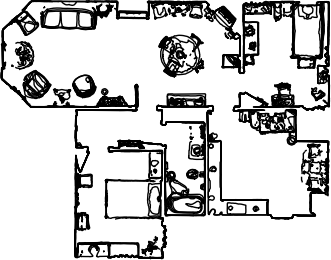
\includegraphics[width=\textwidth]{images/occupancygrid.png}
		\caption{Binary occupancy grid map.}
		\label{fig:binary_grid_map}
	\end{subfigure}
	\hfill
	\begin{subfigure}[b]{0.45\linewidth}
		\centering
		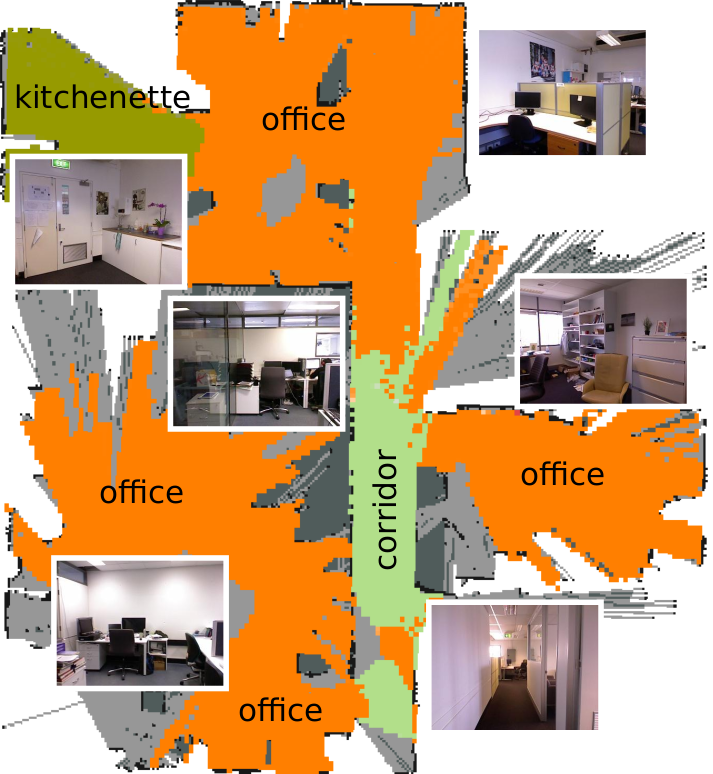
\includegraphics[width=\textwidth]{images/semanticmap.png}
		\caption{Semantic map \cite{placecategorization}.}
		\label{fig:semantic_map}
	\end{subfigure}
	\newline
	\newline
	\begin{subfigure}[b]{0.99\linewidth}
		\centering
		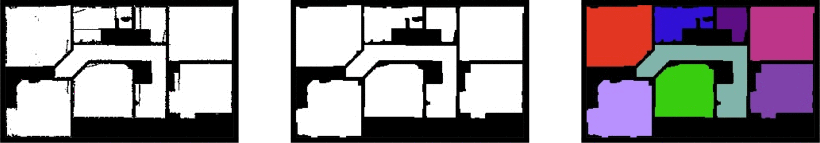
\includegraphics[width=\textwidth]{images/roomsegmentation.png}
		\caption{Room segmentation map \cite{segmentation3d}.}
		\label{fig:room_segmentation_map}
	\end{subfigure}
	\caption{Three different types of maps.}
	
\end{figure}

The room level map obtained through room segmentation can be further improved by exploiting scene recognition or place categorization. This task consists of semantically labeling indoor scenes, such as an ``office'', a ``kitchen'', or a ``bedroom''. Through place categorization, an autonomous agent builds a semantic map (an example is shown by Fig. \ref{fig:semantic_map}), in which any environment location is tagged with a label. In literature, there are a lot of studies concerning place categorization by autonomous agents \cite{scenerecognitionaudio, scenerecognitiononjectdetection, placecategorization, placecategorizationlargescale}. These approaches collect useful information from the scenes (like audio signals or RGB images), then classify these data to divide the environment into rooms, and finally assign a semantic label to each place. One of the main problems is to correctly segment the environment into rooms. This is because data acquired in different rooms can be similar (in this case adjacent rooms can be considered as the same semantic place) or the same room can present different features which can result in an incorrect division of a single room. Identifying the rooms' connections and estimating their location allows mobile robots
to robustly identify different rooms. Furthermore, doors detection can help these methods to find the precise location in which a semantic place ends and another room begins, performing a more refined place segmentation and categorization.  

Another task that can get benefit from doors detection is Semantic SLAM (Simultaneous Localization and Mapping). Semantic SLAM aims to build a semantic map online during exploration without a complete and previously-acquired knowledge of the environment. Recent Semantic SLAM methods combine classical geometry-based estimation with Deep Learning-based object detection. The work presented in \cite{semanticslamsurvey} surveys and evaluates the most relevant approaches that perform Semantic SLAM. The authors argue that semantic segmentation is the largest source of error in the analyzed methods. Doors are useful semantic features of indoor environments and their detection can be added in Semantic SLAM approaches. Furthermore, doors detection can improve the segmentation accuracy performed in previous stages, because the robot can robustly group the data acquired in different rooms. 

Another task that can be improved by exploiting doors recognition is navigation. The authors of \cite{sonarandivisualdoordetection} propose a method to anticipate the door's crossing during navigation, in order to improve the door traversing task. A similar approach is presented in \cite{doorsandnavigation}, where \citeauthor{doorsandnavigation} describe a method for finding doors online during navigation, facilitating how a robot approaches doors. These works prove the usefulness of doors' data for navigation in autonomous agents.

\section{Goals}
\label{sec:goals}
This thesis presents a module to perform doors detection by autonomous mobile robots. As discussed in the previous chapter, Researchers propose feature-based methods \cite{sonarandivisualdoordetection, humanoid, edgeandcornerdoorsdetector} and Deep Learning-based approaches \cite{detectdoorsfeature, doorsandnavigation, doorcabinet} for detecting door in indoor environments.  The module proposed in this work uses RGB images as input data, approaching the problem as an object detection task. Since Computer Vision is highly dependent on the power of Deep Learning \cite{deeplearningoverview} and the novel transformers-based architectures for object detection obtain competitive results \cite{surveytransformer}, the proposed detector is based on DETR \cite{detr}: a deep end-to-end module that take advantages of Transformers to capture the relationships between visual features vectors extracted by a CNN backbone. DETR demonstrates accuracy and run-time performance on par with the well-established and highly-optimized Faster RCNN \cite{fasterrcnn} baseline on the challenging COCO object detection dataset \cite{coco}. Furthermore, DETR does not require any customized layers, and thus can be reproduced easily in any framework that contains standard CNN and transformer classes (like PyTorch\footnote{The PyTorch web page: \url{https://pytorch.org/}.}). Another purpose of this thesis is to test the performance of DETR for doors detection and evaluate the peculiarities of transformers in a Robotic Vision task.

The development and training of a deep module used in a Robotic Vision context have to be as much general as possible. This is because, once deployed, mobbile agents operate in unknown environments. The model's performance can degrade significantly in unfamiliar scenes since their features and structural characteristics have not been considered during the training phase. Despite this, an autonomous agent operates in a few environments during its life cycle. Intelligent agents, like service robots or smart vacuum cleaners, are deployed in a specific environment and often operate inside it for a long time. Frequently moving a robot from a scene to another is not a common scenario. Intelligent agents implement complex strategies for orienting and navigating in real environments. As robots try to understand a scene as well as possible, also artificial environments offer some feature and structural elements that help agents' perception. Researches defined the \textit{wayfinding} principle, which encompasses all of the ways with which people (and animals) orient themselves in physical space and navigate from a place to another. Following this knowledge of how humans perceive, architects and designers build artificial environments that help humans orient and navigate inside them. In \citeyear{imageofcity}, \citeauthor{imageofcity} introduced this concept in his book \citetitle{imageofcity}, where \textit{wayfinding} is defined as ``a consistent use and organization of definite sensory cues from the external environment''.  The author argues that, in the process of \textit{wayfinding}, the strategic link is the generalized mental image of the exterior physical world that is held by an individual. The coherence of the image may arise in several ways. For example, objects can be ordered or remarkable in a scene, so the user recognizes them through its previous experience and the familiarity acquired within the environment. Alternatively, an object seen for the first time is identified because it
conforms to a stereotype already constructed by the observer in other scenes. In \citeyear{wayfinding}, the \textit{wayfinding} concept was further expanded in their book entitled \citetitle{wayfinding} \cite{wayfinding}. This work describes and illustrates how people use both sings and other wayfinding cues to find their way in complex scenes, all explained into practical contexts. 
Indoor environments present a coherent design and a standardized visual aspect in order to help \textit{wayfinding} strategies used by intelligent agents. Following this intuition, there are a few types of doors  the same environment, repeated in different locations. The intuition of this thesis is to exploit the environmental features, that improve \textit{wayfinding} in indoor environments (originally realized for humans), by an autonomous agent. By considering the deployment condition of mobile robots (agents operate in the same territory for a long time) and the coherent design of indoor environments, this work proposes an approach for increasing the doors detector accuracy in unfamiliar environments. The main idea is to specialize the previously trained general doors detector for the specific environment in which the robot operates. This method, called \textit{one-shot incremental learning}, consists of collecting a sub-set of examples from the unfamiliar scene in which the robot will be deployed. Then, the detector is re-trained using these new environment-specific data. In this way, the doors detection module learns how to robustly recognize the new types of doors that characterize the previously unknown deployment environment. Furthermore, this thesis investigates the amount of data required this thesis investigates the amount of data required to achieve a significant performance increase with respect to the general detector.

The power of Deep Learning is limited in vision robotics applications by some problems and challenges that researchers are still investigating \cite{surveydeeplimits}. The datasets used in Computer Vision tasks are not suitable for a robotic context. As Deep Learning is a data hungry technique, they do not contain sufficient data to generalize well the problem's domain they represent. Objects of the same category can look very different depending on the context of usage and the scene's design, so the examples must be collected from several environment types. Due to the fact that a mobile agent can autonomously explore an area, the object images to train a deep robotic detector must be captured from different viewpoints. Furthermore, the locations where data are acquired should be consistent with a possible exploration strategy followed by a mobile robot. Another limitation of the Computer Vision datasets is the lack of negative images. A negative image does not contain any object of interest. This is a shortcoming as an autonomous agent acquires and analyzes a huge amount of images but only a few of them represent positive data. In addition to datasets, also the metrics used in Computer Vision are insufficient to evaluate an end-to-end Robotic Vision module. To overcome the limitations on datasets and metrics, we propose a method for acquiring a visual dataset suitable for a Robotic Vision task. The examples are collected in virtualized heterogeneous environments scanned from real-world. The viewpoints are chosen to simulate an exploration strategy plausible for an active agent. Furthermore, this thesis proposes a novel evaluation method that considers also the negative samples.

\section{Problem Description}

Before proceeding with the detailed discussion of our work, we firstly report some definitions and concepts about the problem addressed by this thesis. In the following paragraphs, we define the ideal deployment scenario in which autonomous agents can benefit from the proposed method. Furthermore, we define the concept of door considered by this thesis, specifying the status that they can assume and the data used for their recognition.

\subsection{The Ideal Deployment Scenario}
\label{sec:deploymentscenario}
This thesis proposes an approach to improve the accuracy of a door detector module used by autonomous agents. The method proposed by this work aims to increase the doors detector's accuracy in a specific deployment scenario of mobile robots. Indoor agents are developed to operate in any environment type. This is because the final context in which a robot works is unknown and can vary a lot. Each environment type has its structural characteristics that vary a lot from each other. Furthermore, built environments of the same type can have a completely different design or visual aspect, depending on the location, the construction budget, or the occupants' culture. Since it's difficult to make assumptions on the type or the visual and structural features of the environments in which a robot is deployed, an autonomous agent must be developed in a general way. Despite this, an indoor mobile robot is typically deployed in a single or in a few spaces and does not change environment very often. This is the typical deployment scenario considered by this thesis. We consider the case in which a robot, to exploit its assigned task, navigates the same environment and finds doors to improve its reasoning abilities. The main idea is to specialize a general module that performs doors detection for a single specific environment, in order to improve its performance. In the context of this thesis, we take into account only indoor environments. In particular, they are a heterogeneous set of multi-floor houses, in which each environment has a particular interior design and a different visual aspect, to better generalize the problem. Furthermore, we assume the environments are static, i.e. their structural features don't change during exploration.

\subsection{Door's Definition and Data Used} 
\label{sec:door_definition}
The second set of definitions we make is about the concept of doors and the data used by the detector to find them. The authors of the work presented in \cite{topologyurban} define the concept of \textit{portal}, which is located whenever a pair of different spaces are adjacent and no physical barriers prevent direct traversals between them.  A portal can be \textit{vertical} or \textit{horizontal}. The first type of portal connects adjacent floors in the same indoor environment (such as stairs, elevators, or ramps), while the latter unifies a tuple of locations on the same floor. The authors identify two types of horizontal portals: \textit{explicit} and \textit{implicit}. Explicit portals are connections between two adjacent spaces that include a barrier (e.g. a doorway through a wall), while implicit portals represent free connections between spaces, with no physical barrier. In the context of this thesis, we consider doors as implicit and explicit horizontal portals. In particular, explicit doors are composed of a jamb and a leaf. Otherwise, implicit doors do not have these components, typically they are only holes in walls that connect different spaces in the same environment. We consider both \textit{internal} and \textit{external} doors. The first are connections between two different spaces inside the same environment while the latter lead out of the building. The method proposed by this thesis not only detects doors but also their status. A door can be \textit{open} or \textit{closed}. A door is closed when the door leaf is completely rested on the jamb, while a door is considered open if it presents even a little hole. We do not consider any other intermediate state (e.g. semi-open) and do not define how much a door is opened. It is important to specify that only explicit doors can assume both statuses, while implicit ones are always open. The approach we describe in this thesis detects doors from RGB images. Doors are highlighted in images by drawing a rectangular bounding box around it.

\begin{figure}[h!]
	\centering
	\begin{subfigure}[b]{\linewidth}
		\centering
		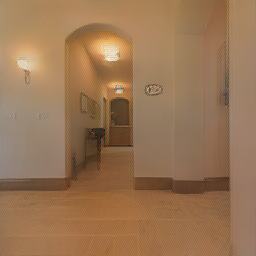
\includegraphics[width=0.24\textwidth]{images/implicitdoor1.png}
		\hfill
		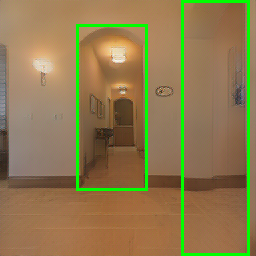
\includegraphics[width=0.24\textwidth]{images/implicitdoor1boxed.png}
		\hfill
		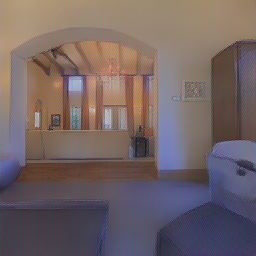
\includegraphics[width=0.24\textwidth]{images/implicitdoor2.png}
		\hfill
		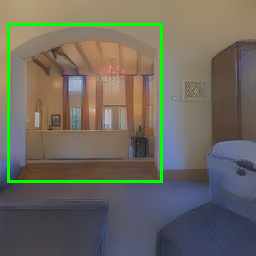
\includegraphics[width=0.24\textwidth]{images/implicitdoor2boxed.png}
		\caption{Implicit internal open doors and the relative bounding boxes.}
	\end{subfigure}
	
	\begin{subfigure}[b]{\linewidth}
		\centering
		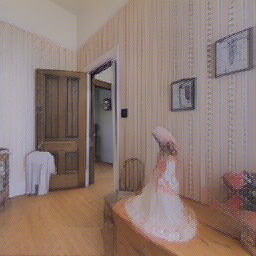
\includegraphics[width=0.24\textwidth]{images/explicitinternalopen1.png}
		\hfill
		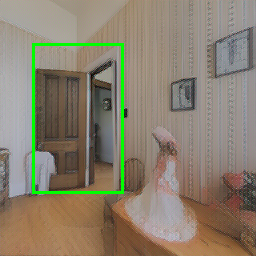
\includegraphics[width=0.24\textwidth]{images/explicitinternalopen1boxed.png}
		\hfill
		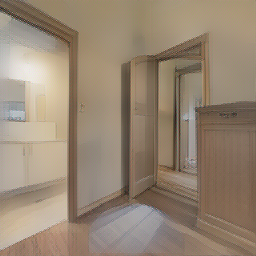
\includegraphics[width=0.24\textwidth]{images/explicitinternalopen2.png}
		\hfill
		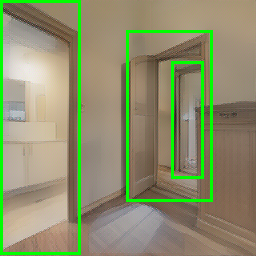
\includegraphics[width=0.24\textwidth]{images/explicitinternalopen2boxed.png}
		\caption{Explicit internal open doors and the relative bounding boxes.}
	\end{subfigure}
	
	\begin{subfigure}[b]{\linewidth}
		\centering
		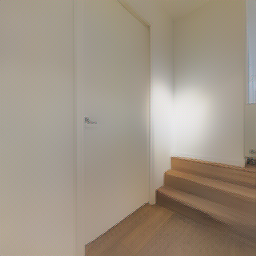
\includegraphics[width=0.24\textwidth]{images/explicitinternalclosed1.png}
		\hfill
		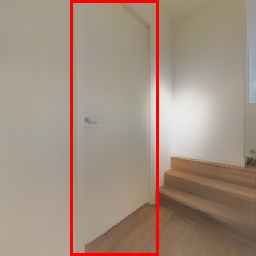
\includegraphics[width=0.24\textwidth]{images/explicitinternalclosed1boxed.png}
		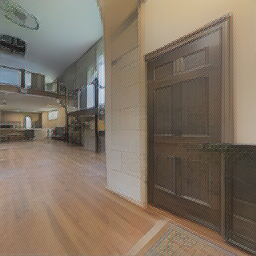
\includegraphics[width=0.24\textwidth]{images/explicitinternalclosed2.png}
		\hfill
		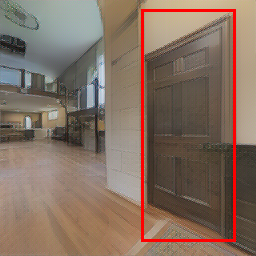
\includegraphics[width=0.24\textwidth]{images/explicitinternalclosed2boxed.png}
		\caption{Explicit internal closed doors and the relative bounding boxes.}	
	\end{subfigure}
	
	\begin{subfigure}[b]{\linewidth}
		\centering
		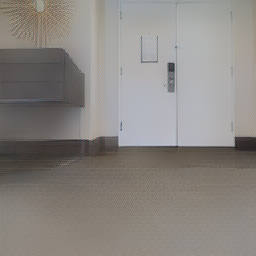
\includegraphics[width=0.24\textwidth]{images/explicitexternalclosed1.png}
		\hfill
		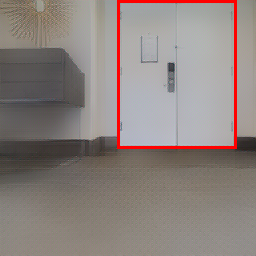
\includegraphics[width=0.24\textwidth]{images/explicitexternalclosed1boxed.png}
		\hfill
		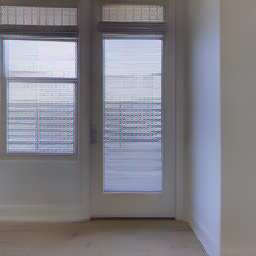
\includegraphics[width=0.24\textwidth]{images/explicitexternalclosed2.png}
		\hfill
		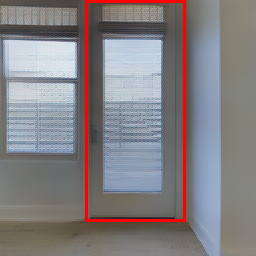
\includegraphics[width=0.24\textwidth]{images/explicitexternalclosed2boxed.png}
		\caption{Explicit external closed doors and the relative bounding boxes.}
	\end{subfigure}
	\caption{Different types of doors with ground truth bounding boxes. Green bounding boxes represent open doorways while red rectangles denote closed doors. These images are taken form Matterport3D \cite{matterport} environments simulated by Gibson \cite{gibson}.}
\end{figure}

\section{Proposed Solution}
\label{sec:solution}
In this thesis, we face the problem of doors detection in autonomous mobile robots. In the following paragraphs, we expose the proposed solutions about the three main problems this work addresses: how to build the doors detector, how to improve the module's performance, and how to compose and evaluate a visual dataset in a robotic vision context.

\paragraph{Build the Doors Detector Module} At first, we reduce to problem of finding doors in indoor environments to a well-known Computer Vision task: object detection in RGB images. After a literature review about this subject, we propose a module to detect doors based on DETR (DEtection TRanformer) \cite{detr}, a deep end-to-end architecture that performs object detection exploiting the Transformers' peculiarities \cite{transformer}. DETR views object detection as a direct set prediction problem, removing the need for many hand-designed components (like non-maximum suppression or anchor generation) that explicitly encode prior knowledge about the task. Thanks to the novel Transformer's architecture, DETR extract features from a frame and then finds the pair-wire relations between them. In this way, it reasons about the entire image as context. The authors demonstrate that DETR accuracy and run-time performance are comparable to the well-established and highly-optimized Faster R-CNN baseline \cite{fasterrcnn} on the challenging COCO object detection dataset \cite{coco}. Despite this, DETR is an enormous network with tens of millions of parameters and it is extremely data-hungry: the authors train DETR for 300 epochs with COCO's examples randomly modified with data augmentation procedures (e.g. resize, crop, scale, etc.). This thesis demonstrates the versatility of DETR with respect to other object detection tasks, even with smaller datasets than COCO.

\paragraph{Increase the Detector's Performance} Another goal of this thesis is to improve the doors detector's accuracy. To address this problem, we do not focus on the deep module that performs object detection, but we reason about its context of use. We focus on a typical deployment scenario for indoor mobile robots (as described in Sec. \ref{sec:deploymentscenario}). We argue that, often, a robot is deployed in a single environment and works inside it for a long time. Furthermore, thanks to  the wayfinding principles described in Sec. \ref{sec:goals}, different views from the same indoor scene presents a coherent visual aspect. This is also true for doors: a single environment presents a few types of doors that are repeated in multiple locations. The method to increase the doors detector's accuracy exploits these intuitions. Our approach, called \textbf{one-shot incremental learning}, aims to specialize the model for working in a precise environment using the fine-tune technique. 

Fine-tuning on pre-trained ImageNet classification models \cite{verydeepimagenet, resnet} has achieved impressive results for tasks such as object detection \cite{fasterrcnn, yolo, yolov2} and is becoming the common way for solving computer vision problems. Fine-tuning is a simple and effective
approach for transfer learning: it concerns training a deep model with common large datasets (such as ImageNet \cite{imagenet} or Microsoft COCO \cite{coco}). Then, the pre-trained model is re-trained with a few new data to solve a more refined task. In this way, the network's weights are set using a source dataset with a large number of examples provide a better
model initialization than random initialization. This is useful to speed up the training, overcome small dataset size, or prevent overfitting. We use the same principle to increase the performance of the proposed doors detector. 

In our approach, called \textbf{one-shot incremental learning}, the doors detector we proposed is initially trained with a general visual doors dataset, which can be downloaded from the internet or collected in some real or simulated environments. The resulting module is a general door detector that can be deployed in any environment. Then, the general detector (built using DETR) is fine-tuned using multiple sub-sets (with different sizes) of new unseen data acquired directly in the new scene. In this way, the general door detector specializes itself using new examples for increasing its performance in a precise environment. Since the fine-tune is performed using multiple sub-sets with different sizes of new data, we also investigate the number of unseen examples necessary to obtain a significant performance improvement.

\paragraph{Compose and Evaluate the Visual Dataset}
This thesis address a Robotic Vision task that completely differs from Computer Vision application. As reported in \cite{surveydeeplimits}, perception is only one part of a more complex, embodied, active, and goal-driven system in robotics.
In a simplified view, whereas Computer Vision takes images and translates them into information, Robotic Vision translates images into actions. Furthermore, an autonomous agent operates in open-set conditions. A module used by a robot can assign high-confidence scores to unknown objects or falsely recognize them as one of the known classes. 

In order to understand how the doors detector performs in different environments, this thesis proposes a method to acquire a dataset of RGB images through simulation. We collect both positive images (that contain doors to detect) and negative frames (that do not depict objects of interest) from multiple scenes. We use Gibson \cite{gibson} to simulate an agent and its visual perception in environments taken from the Matterport3D worlds dataset \cite{matterport}. A mobile robot navigates in an environment following an exploration strategy, avoiding going too close to walls, furniture, and obstacles in general. Furthermore, a robot perceives the environment from different points of view, according to its position in the scene and the height of the camera. To take this fact into account, we propose an approach to select the different locations from which to acquire the data. This method, based on the work presented by \citeauthor{repeatabilityslamarxiv} \cite{repeatabilityslamarxiv, repeatabilityslam}, computes the Voronoi Graph of the occupancy grid maps of an environment. The locations form which to acquire the RGB images are chosen by sub-sampling the Voronoi Graph with a distance value. Thank to this algorithm, the doors dataset is acquired simulating a possible exploration strategy, avoiding collecting wrong or noise images that can degrade the model accuracy.

